% !TEX root = rob1.tex
\chapter{Greifplanung}

\begin{figure}[!h]
    \centering
    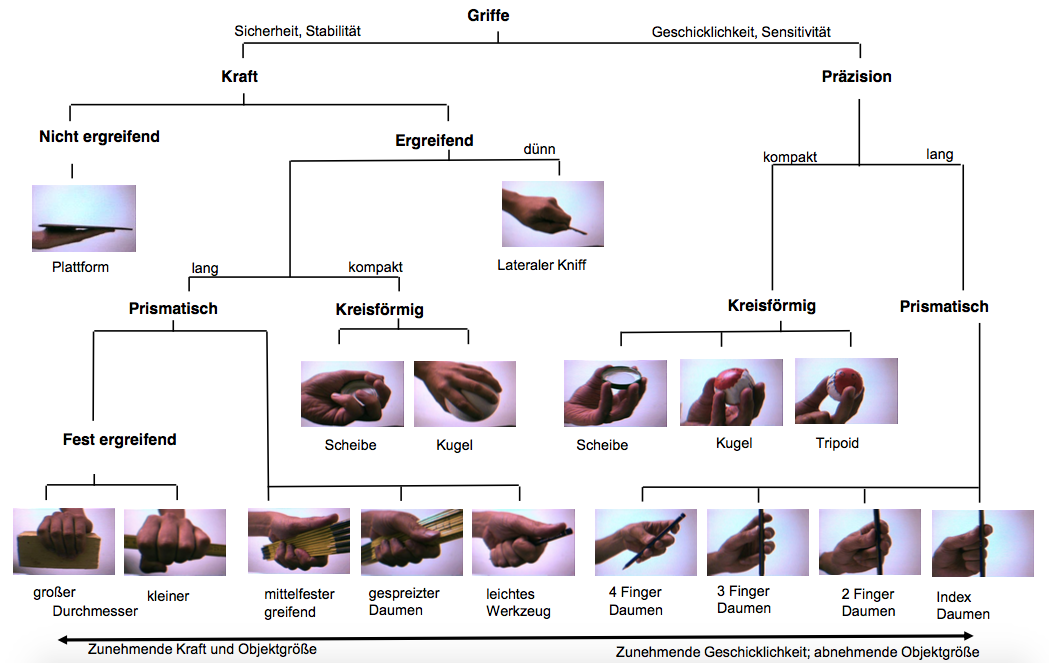
\includegraphics [scale=0.5]{griff}
    \caption{Cutkosky Grifftaxonomie}
\end{figure}

\section{Nebenbedinungen}
\subsection{Intern}
\begin{compactitem}
    \item \textbf{I1: Gültigkeit des Griffes}, Überlappung zwischen den Greifmerkmalen des zu greifenden
    Objektes und den Greifmerkmalen der Greiferfinger
    \item \textbf{I2: Kollisionsfreiheit des Griffes}, keine Kollision zwischen Greifer und gegriffenem
    Objekt
    \item \textbf{I3: Zugänglichkeit des Griffes}, der Griff ist für den Greifer kollisionsfrei erreichbar
\end{compactitem}
\subsection{Extern}
\begin{compactitem}
    \item \textbf{E1: Kollisionsfreie Anrückbewegung des Greifers}, keine Kollision zwischen Roboterarm,
    Grifer, benachbarten Objekten und Arbeitsebene
    \item \textbf{E2: Kollisionsfreie Abrückbewegung mit gegriffenem Objekt}, siehe e1
    \item \textbf{E3: Berücksichtigung der Roboterkinematik}, der selektierte Griff liegt im Arbeitsraum
    des Roboters und die korrespondierenden Trajektorien der Anrück und Abrückbewegung können
    können vom Roboter abgefahren werden.
    \item \textbf{E4: Stabilität des Griffes}, sowohl während der Greifbewegung der Greiferfinger als
    auch während der Transferbewegung des Greifers mit gegriffenem Objekt verändert sich die relative
    Lage und Orientierung des zu greifenden/gegriffenen Objekts zum Greifer nicht
    \item \textbf{E5: Stabilität der Szene}, Abrückbewegung des Greifers mit gegriffenem Objekt sollte
    die Stabilität der Szene nicht beeinflussen.
    \item \textbf{E6: Aufgabenabhängigkeit des Griffs}, wird Pick and Place Operation ausgeführt, dann
    muss zur Aufnahme und Ablagekonfiguration des zu greifenden Objektes kompatibler Griff gewählt werden.
    \begin{compactitem}
        \item Kann kein Griff bestimmt werden, der Nebenbedingung erfüllt, muss geeignete Umgreifsequenz
        bestimmt werden.
        \item Erfordert Griff Ausübung von Kraft und Kraftmomenten auf das Objekt, so muss Greifer diese
        Aufbringen können
    \end{compactitem}
\end{compactitem}

\section{Greifanalyse und Synthese}
\mparagraph{Greifanalyse}
\begin{compactitem}
    \item gegeben: Objekt und Menge von Kontaktpunkten
    \item gesucht: Aussagen zur Stabilität des Giffs unter Berücksichtung der Nebenbedinungen.
\end{compactitem}
\mparagraph{Greifsynthese}
\begin{compactitem}
    \item gegeben: Objekt und eine Menge von Nebenbedinungen.
    \item gesucht: Menge von Kontaktpunkten
\end{compactitem}

\section{Kontaktmodelle}
\begin{compactitem}
    \item Kontakt ohne Reibung (existiert nicht)
    \item Kontakt mit Reibung (Kraft wirkt normal als auch tangential zur Fläche)
    \item Soft-Kontakt (Kraft wirkt normal, tangential. Zusätzlich wirken axiale Momente)
\end{compactitem}
Reibungskegel wird kontinuierlich oder mit approximiert mit Polyeder beschrieben

\mparagraph{Wrenchvektor}
Vektor $\vec{w}$ fasst die in einem Kontaktpunkt $\vec{p}_i$ wirkenden Kräfte $f_i$ und Momente
$\tau_i$ mit $i \in \{x,y,z\}$ zusammen. \\
In Abhängigekeit vom Typ des i-ten Kontaktpunktes normalen \textbf{n}, tangentiale Kräft \textbf{t} und
axiale Momente \textbf{$\Theta$}: $^i\vec{w}_n, ^i\vec{w}_t, ^i\vec{w}_\Theta$ bzw. korrespondierende
Skalare $^ic_n, ^ic_t, ^ic_\Theta$
\mparagraph{Greifmatrix}
Darstellung der Wrenchvektoren für einen räumlichen Griff als Spaltenvektor einer 6 x 3m Matrix G.

\mparagraph{Gleichgewichtsgriff}
Ein Griff wird als Gleichgewichtsgriff bezeichne,t wenn die Summer aller Kräfte $f_i$ und Momente
$\tau_i$, die auf das gegriffene Objekt wirken, gleich Null ist.
\begin{align}
    &1. \forall i \in \{1, ...,m\} : ^ic_n \geq 0, ^i\mu_t * ^ic_n \geq |^ic_t|, ^i\mu_\Theta * ^ic_n
    \geq |^ic_\Theta| \\
    &2. \exists \vec{c} \in R^{3m}, \vec{c} \neq \vec{0} : G.\vec{c} + \vec{e} = 0
\end{align}
$^i\mu_t, ^i\mu_\Theta \in R$ = Coulombschen Reibungskoeffizienten am i-ten Kontaktpunkt
